\documentclass[11pt,a4paper]{article}
\usepackage[margin=1.9cm]{geometry}
\usepackage[T1]{fontenc}
\usepackage{lmodern}
\usepackage{microtype}
\usepackage{amsmath}
\usepackage{xcolor}
\usepackage{booktabs}
\usepackage{tabularx}
\usepackage{array}
\usepackage{enumitem}
\usepackage{float}
\usepackage{tikz}
\usetikzlibrary{arrows.meta,positioning,calc,fit,backgrounds}
\usepackage[colorlinks=true,linkcolor=blue!50!black,urlcolor=blue!50!black]{hyperref}

\setlength{\parindent}{0pt}
\setlength{\parskip}{0.55em}
\setlist{itemsep=0.2em,topsep=0.3em}
\renewcommand{\arraystretch}{1.25}

\definecolor{accent}{HTML}{2F6FB5}
\definecolor{filefill}{HTML}{EEEEEA}
\definecolor{edge}{HTML}{6E6E6A}

% file / script name in typewriter font (underscores are safe)
\newcommand{\fn}[1]{{\ttfamily\detokenize{#1}}}
\newcolumntype{Y}{>{\raggedright\arraybackslash}X}

% ---------- flowchart styles ----------
\tikzset{
  script/.style={rectangle,draw=edge,thick,fill=white,minimum width=4.9cm,minimum height=1.0cm,
                 inner sep=3pt,align=left,font=\scriptsize,text width=4.6cm},
  data/.style={rectangle,rounded corners=5pt,draw=edge,thick,dashed,fill=filefill,minimum width=4.9cm,
                 minimum height=1.0cm,inner sep=3pt,align=left,font=\scriptsize,text width=4.6cm},
  wesad/.style={rectangle,rounded corners=5pt,draw=accent,very thick,dashed,fill=accent!12,
                 minimum width=4.9cm,minimum height=1.0cm,inner sep=3pt,align=left,font=\scriptsize,text width=4.6cm},
  flow/.style={-{Stealth[length=5pt]},edge,thick},
  manual/.style={-{Stealth[length=5pt]},edge,thick,dashed},
  lab/.style={font=\scriptsize\itshape,text=edge}
}
\newcommand{\nm}[2]{\textbf{\ttfamily\detokenize{#1}}\\[-1pt]{\color{black!65}#2}}

\title{\textbf{Pipeline, Labels and Training:\\ WESAD vs.\ Our Users}}
\author{Akshat Priyadarshi (23CS30003)\\ \small Supervisor: Dr.\ Bivas Mitra, IIT Kharagpur}
\date{\today}

\begin{document}
\maketitle

\begin{abstract}
\noindent The final stress model (ContextGate) is trained in two steps on two different datasets.
WESAD (15 lab subjects) teaches the encoder without labels; the survey (STAI-6) answers of our five
wearers train the gate and classifier. This document lists the file behind each step, shows how each
survey answer becomes a label, states which windows were dropped and why, and describes how the model
was trained.
\end{abstract}

%====================================================================
\section{Pipelines at a glance}
%====================================================================
\textbf{WESAD.} Raw files become 7 channels at 1\,Hz, which train the encoder without labels. The
encoder is then frozen and handed to the user pipeline. WESAD's own labels are used only for the audit.

\begin{figure}[H]
\centering
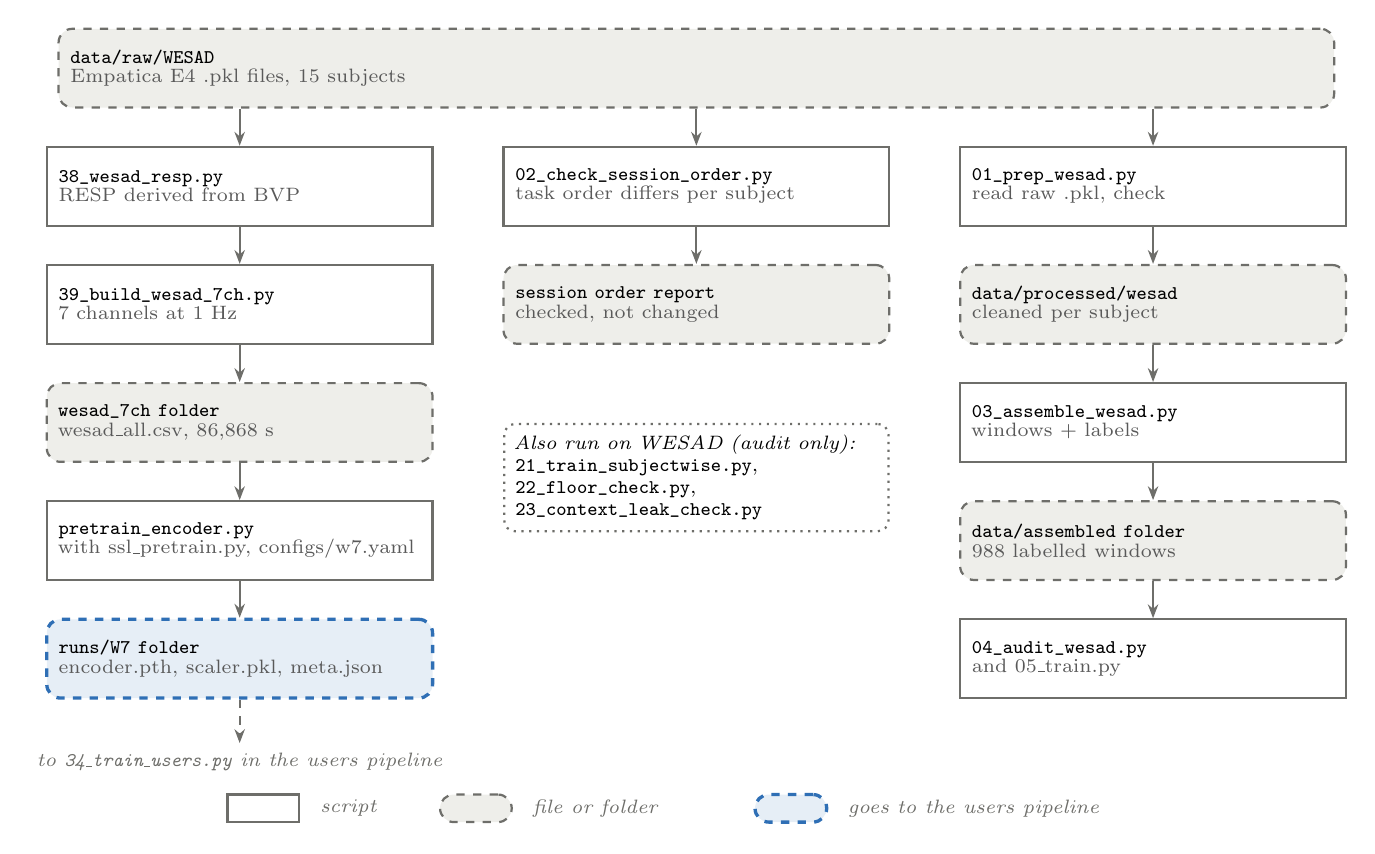
\begin{tikzpicture}[x=1cm,y=1cm]
  % columns at x = 0, 5.8, 11.6 ; rows pitch 1.45
  \node[data,minimum width=16.2cm,text width=15.9cm] (raw) at (5.8,0) {\nm{data/raw/WESAD}{Empatica E4 .pkl files, 15 subjects}};

  % left column: encoder
  \node[script] (s38) at (0,-1.5) {\nm{38_wesad_resp.py}{RESP derived from BVP}};
  \node[script] (s39) at (0,-3.0) {\nm{39_build_wesad_7ch.py}{7 channels at 1 Hz}};
  \node[data]   (f7)  at (0,-4.5) {\nm{wesad_7ch folder}{wesad\_all.csv, 86,868 s}};
  \node[script] (pre) at (0,-6.0) {\nm{pretrain_encoder.py}{with ssl\_pretrain.py, configs/w7.yaml}};
  \node[wesad]  (w7)  at (0,-7.5) {\nm{runs/W7 folder}{encoder.pth, scaler.pkl, meta.json}};

  % middle column: session order
  \node[script] (s02) at (5.8,-1.5) {\nm{02_check_session_order.py}{task order differs per subject}};
  \node[data]   (rep) at (5.8,-3.0) {\nm{session order report}{checked, not changed}};
  \node[draw=edge,dotted,thick,rounded corners=4pt,font=\scriptsize,text width=4.6cm,align=left,inner sep=4pt]
        (also) at (5.8,-5.2) {\textit{Also run on WESAD (audit only):}\\
        \fn{21_train_subjectwise.py}, \fn{22_floor_check.py}, \fn{23_context_leak_check.py}};

  % right column: audit branch
  \node[script] (s01) at (11.6,-1.5) {\nm{01_prep_wesad.py}{read raw .pkl, check}};
  \node[data]   (prc) at (11.6,-3.0) {\nm{data/processed/wesad}{cleaned per subject}};
  \node[script] (s03) at (11.6,-4.5) {\nm{03_assemble_wesad.py}{windows + labels}};
  \node[data]   (asm) at (11.6,-6.0) {\nm{data/assembled folder}{988 labelled windows}};
  \node[script] (s04) at (11.6,-7.5) {\nm{04_audit_wesad.py}{and 05\_train.py}};

  \draw[flow] (raw.south -| s38) -- (s38.north);
  \draw[flow] (raw.south -| s02) -- (s02.north);
  \draw[flow] (raw.south -| s01) -- (s01.north);
  \draw[flow] (s38) -- (s39);
  \draw[flow] (s39) -- (f7);
  \draw[flow] (f7) -- (pre);
  \draw[flow] (pre) -- (w7);
  \draw[flow] (s02) -- (rep);
  \draw[flow] (s01) -- (prc);
  \draw[flow] (prc) -- (s03);
  \draw[flow] (s03) -- (asm);
  \draw[flow] (asm) -- (s04);
  \draw[manual] (w7.south) -- ++(0,-0.55) node[lab,below] {to \texttt{34\_train\_users.py} in the users pipeline};

  % legend
  \begin{scope}[shift={(0,-9.4)}]
    \node[script,minimum width=0.9cm,minimum height=0.35cm,text width=0.7cm] at (0.3,0) {};
    \node[lab,anchor=west] at (0.9,0) {script};
    \node[data,minimum width=0.9cm,minimum height=0.35cm,text width=0.7cm] at (3,0) {};
    \node[lab,anchor=west] at (3.6,0) {file or folder};
    \node[wesad,minimum width=0.9cm,minimum height=0.35cm,text width=0.7cm] at (7,0) {};
    \node[lab,anchor=west] at (7.6,0) {goes to the users pipeline};
  \end{scope}
\end{tikzpicture}
\caption{WESAD pipeline, file by file. Left: the path that builds the frozen encoder. Right: the
reproduction/audit path that uses WESAD's own labels.}
\label{fig:wesad}
\end{figure}

\textbf{Our users.} Three branches (signals, context, labels) are built separately from the raw files
and the survey, then meet in the training step. Raw files also feed the context branch through the
biomarker and derivation scripts. The frozen WESAD encoder reads the signals and the stress score is
computed for every window.

\begin{figure}[H]
\centering
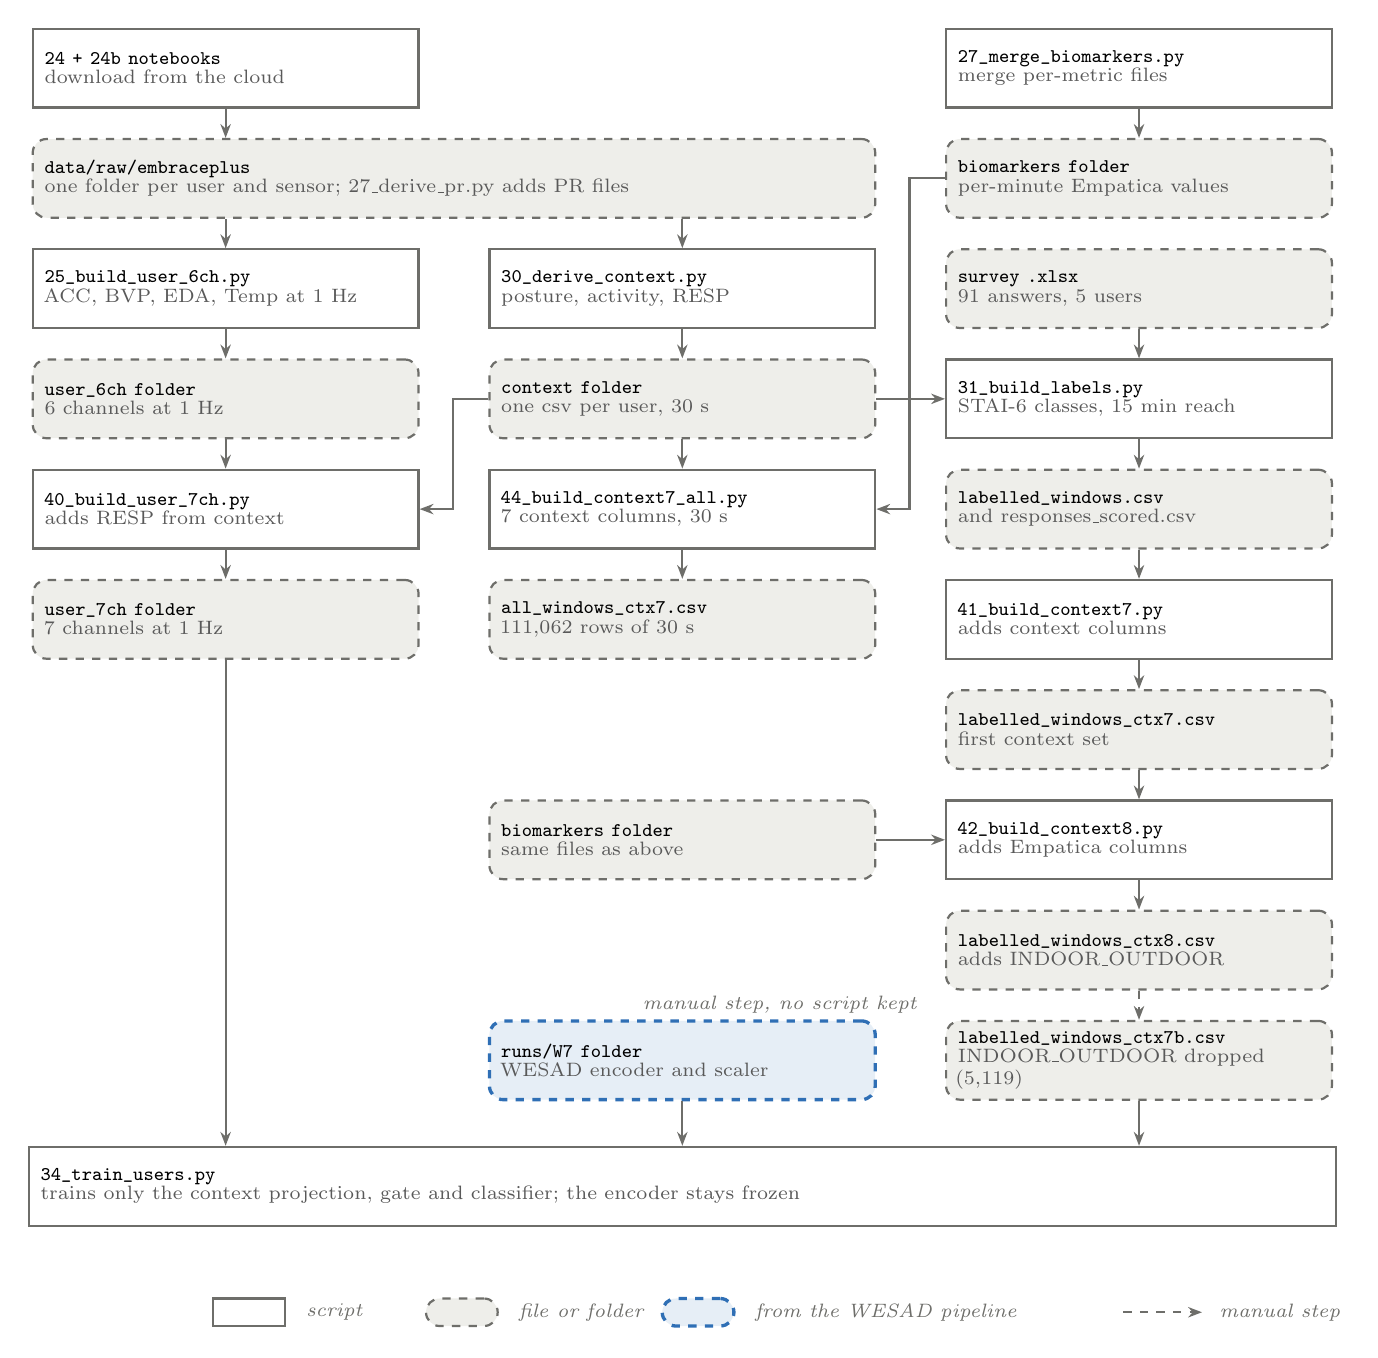
\begin{tikzpicture}[x=1cm,y=1cm]
  % --- row 0
  \node[script] (nb)  at (0,0)    {\nm{24 + 24b notebooks}{download from the cloud}};
  \node[script] (m27) at (11.6,0) {\nm{27_merge_biomarkers.py}{merge per-metric files}};
  % --- row 1
  \node[data,minimum width=10.7cm,text width=10.4cm] (raw) at (2.9,-1.4) {\nm{data/raw/embraceplus}{one folder per user and sensor; 27\_derive\_pr.py adds PR files}};
  \node[data] (bio) at (11.6,-1.4) {\nm{biomarkers folder}{per-minute Empatica values}};
  % --- row 2
  \node[script] (s25) at (0,-2.8)    {\nm{25_build_user_6ch.py}{ACC, BVP, EDA, Temp at 1 Hz}};
  \node[script] (s30) at (5.8,-2.8)  {\nm{30_derive_context.py}{posture, activity, RESP}};
  \node[data]   (sur) at (11.6,-2.8) {\nm{survey .xlsx}{91 answers, 5 users}};
  % --- row 3
  \node[data]   (f6)  at (0,-4.2)    {\nm{user_6ch folder}{6 channels at 1 Hz}};
  \node[data]   (ctx) at (5.8,-4.2)  {\nm{context folder}{one csv per user, 30 s}};
  \node[script] (s31) at (11.6,-4.2) {\nm{31_build_labels.py}{STAI-6 classes, 15 min reach}};
  % --- row 4
  \node[script] (s40) at (0,-5.6)    {\nm{40_build_user_7ch.py}{adds RESP from context}};
  \node[script] (s44) at (5.8,-5.6)  {\nm{44_build_context7_all.py}{7 context columns, 30 s}};
  \node[data]   (lab) at (11.6,-5.6) {\nm{labelled_windows.csv}{and responses\_scored.csv}};
  % --- row 5
  \node[data]   (f7)  at (0,-7.0)    {\nm{user_7ch folder}{7 channels at 1 Hz}};
  \node[data]   (all) at (5.8,-7.0)  {\nm{all_windows_ctx7.csv}{111,062 rows of 30 s}};
  \node[script] (s41) at (11.6,-7.0) {\nm{41_build_context7.py}{adds context columns}};
  % --- rows 6-9 (right column)
  \node[data]   (c7)  at (11.6,-8.4)  {\nm{labelled_windows_ctx7.csv}{first context set}};
  \node[data]   (bio2) at (5.8,-9.8)  {\nm{biomarkers folder}{same files as above}};
  \node[script] (s42) at (11.6,-9.8)  {\nm{42_build_context8.py}{adds Empatica columns}};
  \node[data]   (c8)  at (11.6,-11.2) {\nm{labelled_windows_ctx8.csv}{adds INDOOR\_OUTDOOR}};
  \node[wesad]  (w7)  at (5.8,-12.6)  {\nm{runs/W7 folder}{WESAD encoder and scaler}};
  \node[data]   (c7b) at (11.6,-12.6) {\nm{labelled_windows_ctx7b.csv}{INDOOR\_OUTDOOR dropped (5,119)}};
  % --- training
  \node[script,minimum width=16.6cm,text width=16.3cm] (s34) at (5.8,-14.2)
        {\nm{34_train_users.py}{trains only the context projection, gate and classifier; the encoder stays frozen}};

  % --- arrows
  \draw[flow] (nb) -- (raw.north -| nb);
  \draw[flow] (m27) -- (bio);
  \draw[flow] (raw.south -| s25) -- (s25);
  \draw[flow] (raw.south -| s30) -- (s30);
  \draw[flow] (sur) -- (s31);
  \draw[flow] (s25) -- (f6);
  \draw[flow] (s30) -- (ctx);
  \draw[flow] (f6) -- (s40);
  \draw[flow] (ctx) -- (s44);
  \draw[flow] (s31) -- (lab);
  \draw[flow] (s40) -- (f7);
  \draw[flow] (s44) -- (all);
  \draw[flow] (lab) -- (s41);
  \draw[flow] (s41) -- (c7);
  \draw[flow] (c7) -- (s42);
  \draw[flow] (s42) -- (c8);
  \draw[manual] (c8) -- (c7b);
  \draw[flow] (bio2.east) -- (s42.west);
  \draw[flow] (ctx.east) -- (s31.west);
  \draw[flow] (ctx.west) -- ++(-0.45,0) |- (s40.east);
  \draw[flow] (bio.west) -- ++(-0.45,0) |- (s44.east);
  \draw[flow] (f7.south) -- (f7.south |- s34.north);
  \draw[flow] (w7.south) -- (w7.south |- s34.north);
  \draw[flow] (c7b.south) -- (c7b.south |- s34.north);

  \node[lab,anchor=east] at (8.9,-11.9) {manual step, no script kept};

  % legend
  \begin{scope}[shift={(0,-15.8)}]
    \node[script,minimum width=0.9cm,minimum height=0.35cm,text width=0.7cm] at (0.3,0) {};
    \node[lab,anchor=west] at (0.9,0) {script};
    \node[data,minimum width=0.9cm,minimum height=0.35cm,text width=0.7cm] at (3,0) {};
    \node[lab,anchor=west] at (3.6,0) {file or folder};
    \node[wesad,minimum width=0.9cm,minimum height=0.35cm,text width=0.7cm] at (6,0) {};
    \node[lab,anchor=west] at (6.6,0) {from the WESAD pipeline};
    \draw[manual] (11.4,0) -- (12.4,0);
    \node[lab,anchor=west] at (12.5,0) {manual step};
  \end{scope}
\end{tikzpicture}
\caption{Users pipeline, part 1: from raw recordings and the survey to the training script.
Signals (left), context (middle) and labels (right) are built separately and meet in
\texttt{34\_train\_users.py}.}
\label{fig:users1}
\end{figure}

\begin{figure}[H]
\centering
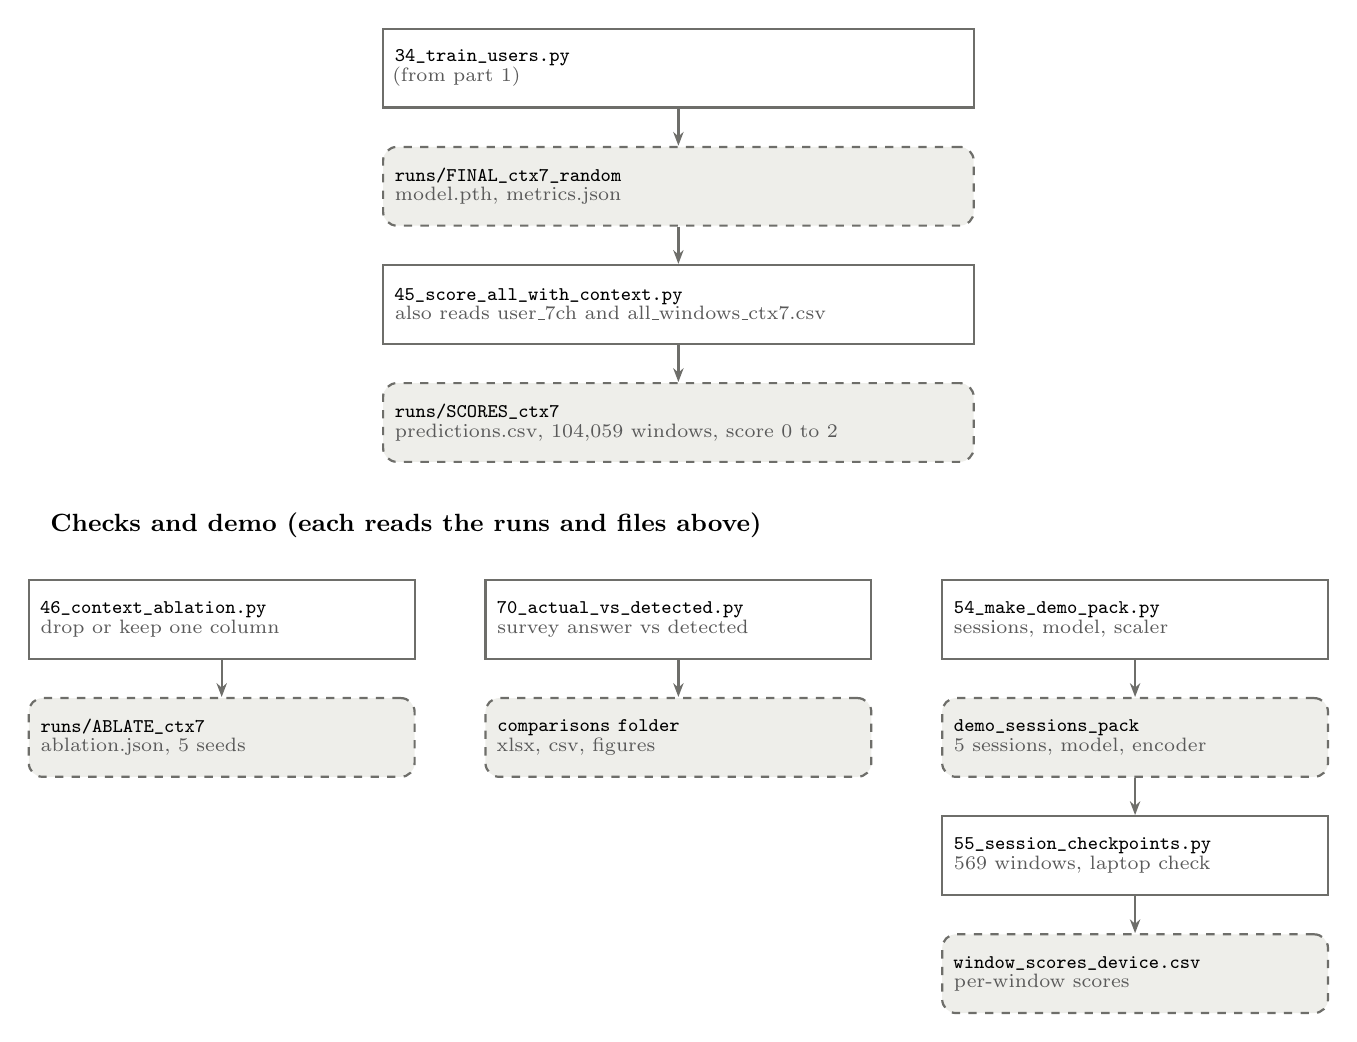
\begin{tikzpicture}[x=1cm,y=1cm]
  \node[script,minimum width=7.5cm,text width=7.2cm] (t) at (5.8,0) {\nm{34_train_users.py}{(from part 1)}};
  \node[data,minimum width=7.5cm,text width=7.2cm]   (fin) at (5.8,-1.5) {\nm{runs/FINAL_ctx7_random}{model.pth, metrics.json}};
  \node[script,minimum width=7.5cm,text width=7.2cm] (s45) at (5.8,-3.0) {\nm{45_score_all_with_context.py}{also reads user\_7ch and all\_windows\_ctx7.csv}};
  \node[data,minimum width=7.5cm,text width=7.2cm]   (sc) at (5.8,-4.5) {\nm{runs/SCORES_ctx7}{predictions.csv, 104,059 windows, score 0 to 2}};
  \draw[flow] (t) -- (fin); \draw[flow] (fin) -- (s45); \draw[flow] (s45) -- (sc);

  \node[font=\small\bfseries,anchor=west] at (-2.3,-5.8) {Checks and demo (each reads the runs and files above)};
  \node[script] (s46) at (0,-7.0)    {\nm{46_context_ablation.py}{drop or keep one column}};
  \node[script] (s70) at (5.8,-7.0)  {\nm{70_actual_vs_detected.py}{survey answer vs detected}};
  \node[script] (s54) at (11.6,-7.0) {\nm{54_make_demo_pack.py}{sessions, model, scaler}};
  \node[data]   (ab)  at (0,-8.5)    {\nm{runs/ABLATE_ctx7}{ablation.json, 5 seeds}};
  \node[data]   (cmp) at (5.8,-8.5)  {\nm{comparisons folder}{xlsx, csv, figures}};
  \node[data]   (pk)  at (11.6,-8.5) {\nm{demo_sessions_pack}{5 sessions, model, encoder}};
  \node[script] (s55) at (11.6,-10.0){\nm{55_session_checkpoints.py}{569 windows, laptop check}};
  \node[data]   (dev) at (11.6,-11.5){\nm{window_scores_device.csv}{per-window scores}};
  \draw[flow] (s46) -- (ab); \draw[flow] (s70) -- (cmp); \draw[flow] (s54) -- (pk);
  \draw[flow] (pk) -- (s55); \draw[flow] (s55) -- (dev);
\end{tikzpicture}
\caption{Users pipeline, part 2: training output, the stress score for every window, and the checks
and demo scripts.}
\label{fig:users2}
\end{figure}

%====================================================================
\section{The pipeline, stage by stage}
%====================================================================
WESAD and our wearers share the same 7 channels, the same 60\,s windows (stride 30\,s) and the same
encoder. They differ in who provides labels and context and in what each dataset is used for: WESAD
builds the encoder, our users train and test the stress score.

\begin{table}[H]
\centering\footnotesize
\begin{tabularx}{\textwidth}{@{}>{\raggedright\arraybackslash}p{2.5cm}YY@{}}
\toprule
\textbf{Stage} & \textbf{WESAD (15 lab subjects)} & \textbf{Our users (5 labelled wearers)}\\
\midrule
1. Raw data & Empatica E4 \fn{.pkl} files. Checked by \fn{s0_check_wesad_raw.py}, \fn{01_prep_wesad.py}, \fn{02_check_session_order.py} (task order differs between subjects)
 & EmbracePlus raw CSVs, downloaded by \fn{24_download_embraceplus.ipynb} and \fn{24b_download_remaining_users.ipynb}\\
2. Signals at 1\,Hz & \fn{39_build_wesad_7ch.py}: ACC x/y/z, BVP, EDA, Temp from the wrist, 86,868 seconds, 15 subjects
 & \fn{25_build_user_6ch.py} (ACC x/y/z, BVP, EDA, Temp), pulse rate from \fn{27_derive_pr.py}\\
3. Breathing channel (RESP) & \fn{38_wesad_resp.py}, derived from BVP, checked against the chest belt ($r=0.185$)
 & \fn{40_build_user_7ch.py} adds RESP, output \fn{user_7ch/<user>.csv} (7 channels)\\
4. Context (7 columns) & Not used in the final model. Only tested for leakage: \fn{23_context_leak_check.py} (Task alone scores 1.000)
 & \fn{27_merge_biomarkers.py}, \fn{30_derive_context.py}, \fn{44_build_context7_all.py}: HOUR, IS\_WEEKEND, POSTURE, ACT\_COUNT, ACT\_CLASS, BODY\_POSITION, SLEEP. Output \fn{all_windows_ctx7.csv} (111,062 rows of 30\,s)\\
5. Labels & Not used in the final model. WESAD's own conditions (baseline $=$ Low, amusement $=$ Medium, stress $=$ High) in \fn{39_build_wesad_7ch.py}, used only for the reproduction and audit
 & \fn{31_build_labels.py}: STAI-6 answers become Low / Medium / High, attached to windows within 15\,min (\fn{labelled_windows.csv}). Then \fn{41_build_context7.py} and \fn{42_build_context8.py} add the context columns, and INDOOR\_OUTDOOR is dropped by hand (no script kept) to give \fn{labelled_windows_ctx7b.csv} (5,119 windows)\\
6. Encoder & \fn{pretrain_encoder.py} and \fn{ssl_pretrain.py} with \fn{configs/w7.yaml}: contrastive, no labels, 2,894 windows. Output \fn{runs/W7/encoder.pth}, \fn{scaler.pkl}, \fn{meta.json}. Then frozen
 & Not trained. The frozen WESAD encoder and WESAD scaler are applied unchanged\\
7. Gate and classifier & Only for the audit (\fn{05_train.py}, \fn{21_train_subjectwise.py}, \fn{22_floor_check.py})
 & \fn{34_train_users.py}: trains only the context projection, gate and classifier on the labelled windows. Output \fn{runs/FINAL_ctx7_random/model.pth}\\
8. Stress score & Not produced
 & \fn{45_score_all_with_context.py}: every window gets $P(\text{Low}),P(\text{Med}),P(\text{High})$ and score $=P(\text{Med})+2P(\text{High})$, 0 to 2. Output \fn{runs/SCORES_ctx7/predictions.csv} (104,059 windows)\\
9. Checks and demo & \fn{04_audit_wesad.py}
 & \fn{46_context_ablation.py}, \fn{70_actual_vs_detected.py}, then \fn{55_session_checkpoints.py} on the five demo sessions and the Jetson\\
\bottomrule
\end{tabularx}
\caption{Stage-by-stage file map. The two columns meet at stage 6: the encoder built from WESAD is what the user pipeline reads in stage 7.}
\end{table}

%====================================================================
\section{How a survey answer becomes a label}
%====================================================================
Each of the 91 answers is scored, put into one of three classes, and then copied onto every 30\,s
window within 15 minutes either side of the moment it was given. Windows that no answer reaches stay
unlabelled and are not used for training. All of this is in \fn{31_build_labels.py}.

\paragraph{Step 1: score the answer (STAI-6).} Six items are rated 1 to 4: calm, tense, upset, relaxed,
content, worried. Calm, relaxed and content are reversed ($5-$rating). Add the six to get a raw score of
6 to 24, then multiply by $20/6$ to get the STAI-6 score on a 20 to 80 scale.

\paragraph{Step 2: cut into three classes across everyone.} The two cut points (46.67 and 56.67) are the
$1/3$ and $2/3$ quantiles of all 91 scores, not of each person's own scores.

\begin{table}[H]
\centering\small
\begin{tabular}{@{}lllrr@{}}
\toprule
Class & STAI-6 score & Raw score & Answers & Windows\\
\midrule
Low    & up to 46.67     & 14 or less & 33 & 1,949\\
Medium & 46.67 to 56.67  & 15 to 16   & 27 & 1,567\\
High   & 56.67 and above & 17 or more & 31 & 1,603\\
\bottomrule
\end{tabular}
\end{table}

Cutting across everyone means a score of 60 is the same class whoever reported it. WESAD's per-person
cut caused S11's calm baseline to become Medium and S14's to become High.

\paragraph{Step 3: attach the answer to windows ($\pm 15$ minutes).} The context file has one row every
30\,s for as long as the watch was worn. For each user, every row is matched to the nearest answer in
time (\texttt{pd.merge\_asof}, \texttt{direction='nearest'}, tolerance 15\,min). If that answer is within
15 minutes, the row gets the answer's score and class; if not, the row gets no label.

\begin{figure}[H]
\centering
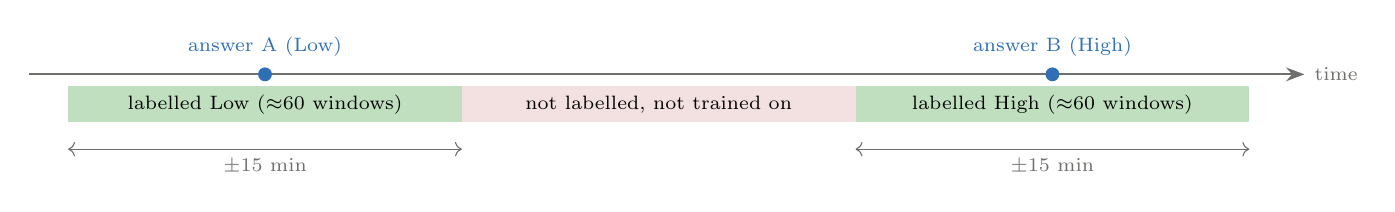
\begin{tikzpicture}[x=1cm,y=1cm]
  \draw[-{Stealth},thick,edge] (0,0) -- (16.2,0) node[right,font=\scriptsize] {time};
  \fill[accent] (3,0) circle (2.5pt) node[above=3pt,font=\scriptsize] {answer A (Low)};
  \fill[accent] (13,0) circle (2.5pt) node[above=3pt,font=\scriptsize] {answer B (High)};
  \fill[green!50!black,opacity=0.25] (0.5,-0.6) rectangle (5.5,-0.15);
  \fill[green!50!black,opacity=0.25] (10.5,-0.6) rectangle (15.5,-0.15);
  \fill[red!60!black,opacity=0.12] (5.5,-0.6) rectangle (10.5,-0.15);
  \node[font=\scriptsize] at (3,-0.38) {labelled Low ($\approx$60 windows)};
  \node[font=\scriptsize] at (13,-0.38) {labelled High ($\approx$60 windows)};
  \node[font=\scriptsize,align=center] at (8,-0.38) {not labelled, not trained on};
  \draw[<->,edge] (0.5,-0.95) -- (5.5,-0.95) node[midway,below,font=\scriptsize] {$\pm$15 min};
  \draw[<->,edge] (10.5,-0.95) -- (15.5,-0.95) node[midway,below,font=\scriptsize] {$\pm$15 min};
\end{tikzpicture}
\caption{Each answer labels the windows within 15 minutes; windows in the gap stay unlabelled.}
\end{figure}

\begin{itemize}
\item \textbf{About 60 windows per answer.} 30 minutes at 30\,s steps is 60 rows. The 88 matched answers
average 58.2 windows each (range 29 to 60); the shorter ones are probably where the watch was off or the
recording started or ended.
\item \textbf{If two answers are close,} each window takes the nearer one. In practice this almost never
happens: the median gap between a person's answers is 244 minutes and only one pair is within 30 minutes.
\item \textbf{Between answers.} Any window more than 15 minutes from every answer is left unlabelled. It
is not guessed, filled in or interpolated, because there is no ground truth. These windows are not used
for training, but they are still scored at inference (stage 8): 104,059 windows get a score, only 5,119
carry a label (about 5\,\%).
\item \textbf{Why 15 minutes and not more.} The survey asks about the last hour, so one answer describes a
stretch of time. A wider reach would make more windows share one label and look like copies of each other
rather than separate examples.
\end{itemize}

\textbf{Result:} 91 answers, 88 matched, 5,119 labelled windows. Per person: user17 13 answers (705
windows), user18 31 (1,649), user25 23 (1,329), user26 18 (1,076), user27 6 (360).

%====================================================================
\section{How context and signals sit under each label}
%====================================================================
A labelled window is one row in the labelled file. It carries the label, the 7 context columns and a
timestamp. The 60\,s of signal underneath it is looked up from the 1\,Hz channel file by that timestamp,
in \fn{load_windows} inside \fn{34_train_users.py}.

\begin{table}[H]
\centering\footnotesize
\begin{tabularx}{\textwidth}{@{}>{\raggedright\arraybackslash}p{1.6cm}YY@{}}
\toprule
\textbf{Part} & \textbf{Where it comes from} & \textbf{What the model reads}\\
\midrule
Label & \fn{31_build_labels.py}: the nearest answer within 15\,min & Class 0, 1 or 2 (Low, Medium, High), the training target\\
Context & \fn{41_build_context7.py} and \fn{42_build_context8.py} add the columns to the labelled windows, then INDOOR\_OUTDOOR is dropped (\fn{labelled_windows_ctx7b.csv}). \fn{44_build_context7_all.py} builds the same columns for every 30\,s row (\fn{all_windows_ctx7.csv}), used for scoring. Matched on the window's 30\,s timestamp
 & HOUR, IS\_WEEKEND, ACT\_COUNT as numbers; POSTURE, ACT\_CLASS, BODY\_POSITION, SLEEP as words. After one-hot encoding this is 19 numbers, fitted on the training rows only\\
Signal & \fn{user_7ch/<user>.csv}, the 60 rows starting at the window's timestamp & $7\times 60$ seconds, scaled with the WESAD scaler, read by the frozen encoder\\
\bottomrule
\end{tabularx}
\end{table}

\textbf{Context source for each column.}
\begin{itemize}
\item HOUR and IS\_WEEKEND come from the timestamp (IST).
\item POSTURE and ACT\_COUNT are derived by us from the wrist accelerometer (\fn{30_derive_context.py}).
\item ACT\_CLASS, BODY\_POSITION and SLEEP are Empatica biomarkers, one value per minute, held across the
two 30\,s steps. Where Empatica recorded nothing the value is the word \textit{Unknown}, so the row is kept.
\end{itemize}
The label and the context are both attached to the same 30\,s timestamp, so the context describes the
moment of the window, while the label describes the answer given within 15 minutes of it.

%====================================================================
\section{What was dropped or ignored, and why}
%====================================================================
Our users: 5,119 labelled windows start from 111,062 context rows. Most rows are left unlabelled because
no answer is near them. Only a few windows and answers are actively thrown away.

\paragraph{Our users}
\begin{table}[H]
\centering\footnotesize
\begin{tabularx}{\textwidth}{@{}YlY@{}}
\toprule
\textbf{What} & \textbf{How many} & \textbf{Why}\\
\midrule
Windows more than 15\,min from every answer & about 105,900 of 111,062 (over 95\,\%) & No ground truth. Not guessed or interpolated. Not used for training, but scored at inference (104,059 scored windows)\\
Answers with no window in reach (all user18: 4 Aug 16:16, 5 Aug 14:23, 10 Aug 11:07; all High, 60 to 63) & 3 of 91 answers, 88 matched & No context rows within 15\,min, so nothing to label. Not forced\\
Labelled windows without 60 contiguous seconds of signal & about 68 (5,119 down to about 5,051, inferred from split sizes 3,536 + $\approx$505 + 1,010) & \fn{load_windows} keeps a window only if 60 consecutive seconds exist (span within $\pm5$\,s) and it does not run past the end of the file\\
Missing samples inside a kept window & not dropped & Filled by interpolation; anything still missing after scaling becomes 0\\
Missing Empatica biomarker (watch off or loose) & not dropped & The cell becomes \textit{Unknown}. The state really is unknown, so the row stays\\
Context columns removed (not rows) & INDOOR\_OUTDOOR, PRV\_RMSSD, AROUSAL\_AT\_REST & INDOOR\_OUTDOOR is a survey answer present at under 1\,\% of windows. PRV\_RMSSD had implausible beat timing (about 290\,ms against 20 to 50\,ms normal). AROUSAL\_AT\_REST was 0.90 correlated with pulse rate\\
Survey rows without user id, timestamp, or with an item outside 1 to 4 & the script would drop them & The 91 responses used were all valid\\
The 10\,\% validation share in the pooled split & about 505 windows & Set aside by the split and not used to choose anything\\
\bottomrule
\end{tabularx}
\end{table}

\paragraph{WESAD}
\begin{table}[H]
\centering\footnotesize
\begin{tabularx}{\textwidth}{@{}YlY@{}}
\toprule
\textbf{What} & \textbf{How many} & \textbf{Why}\\
\midrule
Meditation and transition seconds (condition labels) & 16,136 rows dropped, 30,349 kept & Not baseline, amusement or stress, so a three-class label cannot be made. Only used for the audit\\
Windows spanning two subjects in pretraining & 27 of 2,894 & The repository's windowing does not split by subject. Left unchanged and reported. Kept, not dropped\\
Labelled windows & 988, split by subject & The labelled step splits by subject, so a window never mixes two people\\
\bottomrule
\end{tabularx}
\end{table}
WESAD's labelled windows are not part of the final user model.

%====================================================================
\section{How the model was trained}
%====================================================================
Two training steps use two different datasets. The encoder never sees a label. The classifier never
sees WESAD.

\begin{table}[H]
\centering\footnotesize
\begin{tabularx}{\textwidth}{@{}>{\raggedright\arraybackslash}p{2.2cm}YY@{}}
\toprule
 & \textbf{Step A: encoder (WESAD)} & \textbf{Step B: gate and classifier (our users)}\\
\midrule
Script & \fn{pretrain_encoder.py} $\to$ \fn{ssl_pretrain.py}, \fn{configs/w7.yaml} & \fn{34_train_users.py}\\
Data & \fn{wesad_all.csv}: every second of all 15 subjects, 7 channels & \fn{labelled_windows_ctx7b.csv} (5,119 windows) paired with \fn{user_7ch/} signals\\
Labels & None (self-supervised) & STAI-6 class of the nearest answer within 15\,min: Low, Medium, High\\
Context & None & 7 columns, 19 numbers after one-hot, fitted on the training rows only\\
Signal & 2,894 windows of $7\times60$\,s (stride 30\,s). WESAD scaler fitted here & $7\times60$\,s per window, scaled with that same WESAD scaler\\
Trained & Conv1d$\times3$ + BiLSTM encoder and projection head; 20 epochs, batch 128, Adam $10^{-3}$, NT-Xent ($\tau=0.5$), loss 4.38 $\to$ 3.64 & Context projection, gate and classifier only: 177,795 weights; cross-entropy, Adam $10^{-3}$, batch 64, 20 epochs\\
Frozen & Nothing & The encoder (357,760 weights)\\
Output & \fn{runs/W7/encoder.pth}, \fn{scaler.pkl}, \fn{meta.json} & \fn{runs/FINAL_ctx7_random/model.pth}, \fn{metrics.json}\\
\bottomrule
\end{tabularx}
\end{table}

\paragraph{Contrastive step, in one line.} Each window is shown twice with a small random scale (0.9 to
1.1) and noise (0.01). The encoder is trained so the two versions of the same window land close together
and different windows land apart.

\paragraph{Model architecture for one window.}
\begin{figure}[H]
\centering
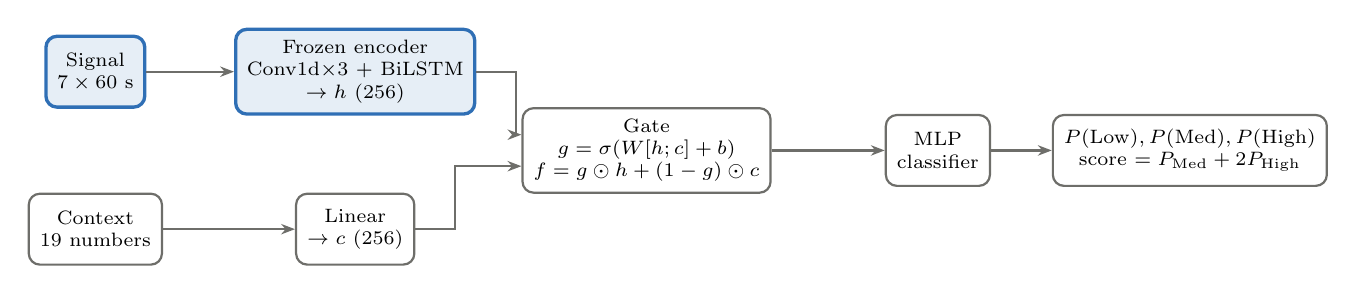
\begin{tikzpicture}[x=1cm,y=1cm,
  blk/.style={rectangle,rounded corners=4pt,draw=edge,thick,fill=white,font=\scriptsize,align=center,minimum height=0.9cm,inner sep=4pt},
  frz/.style={blk,draw=accent,fill=accent!12,very thick}]
  \node[frz] (sig) at (0,1.0) {Signal\\$7\times60$ s};
  \node[frz] (enc) at (3.3,1.0) {Frozen encoder\\Conv1d$\times3$ + BiLSTM\\$\to h$ (256)};
  \node[blk] (ctx) at (0,-1.0) {Context\\19 numbers};
  \node[blk] (prj) at (3.3,-1.0) {Linear\\$\to c$ (256)};
  \node[blk] (gate) at (7.0,0) {Gate\\$g=\sigma(W[h;c]+b)$\\$f=g\odot h+(1-g)\odot c$};
  \node[blk] (mlp) at (10.7,0) {MLP\\classifier};
  \node[blk] (out) at (13.9,0) {$P(\mathrm{Low}),P(\mathrm{Med}),P(\mathrm{High})$\\score $=P_{\mathrm{Med}}+2P_{\mathrm{High}}$};
  \draw[flow] (sig)--(enc); \draw[flow] (ctx)--(prj);
  \draw[flow] (enc.east) -- ++(0.5,0) |- ([yshift=0.2cm]gate.west);
  \draw[flow] (prj.east) -- ++(0.5,0) |- ([yshift=-0.2cm]gate.west);
  \draw[flow] (gate)--(mlp); \draw[flow] (mlp)--(out);
\end{tikzpicture}
\caption{ContextGate for one window. Blue boxes are frozen WESAD components. Trainable: 177,795
weights; total 535,555 ($\approx$2.14\,MB).}
\end{figure}

\paragraph{How the supervised step is split.} The \texttt{--split} option chooses the question being asked:

\begin{table}[H]
\centering\small
\begin{tabularx}{\textwidth}{@{}>{\raggedright\arraybackslash}p{4.2cm}YY@{}}
\toprule
\textbf{Split} & \textbf{What is held out} & \textbf{Question answered}\\
\midrule
random (the final saved model) & Random 70/10/20 of windows, 5 seeds & Can it recall? Near-identical windows of one answer fall on both sides, so this is recall\\
response & Whole survey answers kept on one side & Can it score an answer it has not seen?\\
user & One person held out, rotating & Does it work on a new person?\\
temporal & Each person's earlier answers train, later ones test & Can it score the future?\\
\bottomrule
\end{tabularx}
\end{table}

The saved model uses the random split: 3,536 training windows and 1,010 test windows (seed 42), balanced
accuracy 0.841 averaged over 5 seeds. That number is \emph{not} evidence of prediction: on answers or
people the model has not seen, it does not reliably beat guessing.

\paragraph{WESAD separately.} WESAD teaches the encoder what 60\,s of wrist signal looks like. Its own
labels (baseline, amusement, stress) were used in separate runs only to reproduce and audit the published
result: 0.935 on a random split, 0.800 with overlapping windows kept together, and 0.567 for the deep model
on unseen subjects. Task as context alone gave 1.000, which is leakage: the task is the session, and the
session is the label.

%====================================================================
\section{Limits of these labels, said plainly}
%====================================================================
\begin{itemize}
\item \textbf{One answer is copied onto about 60 windows.} They overlap by 30\,s and look alike, so the
effective number of independent examples is 88 answers, not 5,119 windows.
\item \textbf{The answer describes the last hour,} but is attached to a 30-minute stretch centred on the
moment it was given.
\item \textbf{Five people only, and they used the scale differently.} user26 answered Low all 18 times,
user18 never answered Low, user27 only Low and High. A model trained on four people does not carry over
to the fifth.
\item \textbf{Classes are cut across everyone.} That keeps a score of 60 meaning the same thing for each
person, but a person's own calm baseline can sit in the Medium class.
\item \textbf{Unlabelled windows are not evidence of calm.} The 105,900 windows between answers have no
label at all; they are only scored.
\end{itemize}

\end{document}
